\documentclass[10pt]{article}
\usepackage[a4paper,margin=14mm,top=12mm,bottom=12mm]{geometry}
\usepackage{fontspec}
\setmainfont{TeX Gyre Heros}
\usepackage{graphicx,tikz,array,tabularx,enumitem,multicol,booktabs}
\usepackage[most]{tcolorbox}
\usepackage{xcolor}
\usepackage{amssymb}
\pagestyle{empty}
\setlength{\parindent}{0pt}
\setlength{\parskip}{3pt}
\setlist{nosep,leftmargin=*}
\frenchspacing
\newcommand{\sh}{$\sharp$}
\newcommand{\fl}{$\flat$}

% ---------- headings
\newcommand{\sect}[1]{\par\vspace{5pt}{\large\bfseries #1}\par\vspace{2pt}}

% ---------- drill header
\newcommand{\drill}[6]{%
\noindent
\begin{tikzpicture}[baseline=(b.base)]
\node[fill=black,minimum width=15mm,minimum height=15mm,text=white,inner sep=0,rounded corners=1pt] (b) {};
\node[text=white,font=\sffamily\bfseries\tiny] at ([yshift=-2.3mm]b.north) {DRILL};
\node[text=white,font=\sffamily\bfseries\fontsize{24}{24}\selectfont] at ([yshift=-1.5mm]b.center) {#1};
\end{tikzpicture}\hspace{4mm}%
\begin{minipage}[b]{0.86\textwidth}
{\fontsize{20}{22}\selectfont\bfseries #2}\\[1pt]
{\itshape #3}\\[1pt]
{\small\textbf{Needs:} #4\quad \textbf{Skills:} #5\quad \textbf{Gate:} #6}
\end{minipage}\par\vspace{2pt}
\noindent\rule{\textwidth}{0.8pt}\par\vspace{3pt}}

\newtcolorbox{why}{enhanced,colback=white,colframe=black,boxrule=0.5pt,arc=2mm,
  colbacktitle=black!12,coltitle=black,fonttitle=\small\bfseries,title=Why this matters,
  left=2mm,right=2mm,top=1.5mm,bottom=1.5mm,before skip=2pt,after skip=4pt}
\newtcolorbox{sidebox}[1]{enhanced,colback=white,colframe=black,boxrule=0.5pt,arc=2mm,
  colbacktitle=black!12,coltitle=black,fonttitle=\small\bfseries,title=#1,
  left=2mm,right=2mm,top=1mm,bottom=1mm,fontupper=\small,equal height group=bottom\thepage}
\newtcolorbox{greybox}{enhanced,colback=black!6,colframe=black!6,arc=2mm,left=2mm,right=2mm,top=1mm,bottom=1mm,fontupper=\small}

% ---------- 5 minutes
\newcommand{\tm}[1]{\fbox{\scriptsize\bfseries\strut #1}}
\newenvironment{fivemin}{\sect{The 5 minutes}\small\renewcommand{\arraystretch}{1.25}\tabularx{\textwidth}{@{}p{17mm}X@{}}}{\endtabularx}

% ---------- ladder
\newcommand{\cb}{\framebox(7,7){}}
\newenvironment{ladder}{\begin{tcolorbox}[enhanced,colback=white,colframe=black,boxrule=0.8pt,arc=2mm,
  colbacktitle=black!12,coltitle=black,fonttitle=\small\bfseries,
  title={Level ladder --- stay on a level for days or weeks; tick it when you play it clean 3 times in a row},
  left=0mm,right=0mm,top=0.5mm,bottom=0.5mm,before skip=4pt,after skip=4pt]\small
  \renewcommand{\arraystretch}{1.12}\begin{tabular}{@{\hspace{1mm}}c@{\hspace{1.5mm}}l@{\hspace{1.5mm}}p{0.745\linewidth} r@{\hspace{2mm}}p{13mm}@{}}}
  {\end{tabular}\end{tcolorbox}}
\newcommand{\lv}[3]{\cb & \textbf{#1} & #2 & \footnotesize #3 & \rule[-1pt]{13mm}{0.4pt}\\}

\newcommand{\bottom}[2]{\par\vspace{2pt}\noindent
\begin{tcbraster}[raster columns=2,raster equal height,raster column skip=3mm,
  enhanced,colback=white,colframe=black,boxrule=0.5pt,arc=2mm,colbacktitle=black!12,coltitle=black,
  fonttitle=\small\bfseries,left=2mm,right=2mm,top=1mm,bottom=1mm,fontupper=\small]
\begin{tcolorbox}[title=Make it harder]#1\end{tcolorbox}
\begin{tcolorbox}[title=In the recording]#2\end{tcolorbox}
\end{tcbraster}}

\newcommand{\blank}[1][25mm]{\rule[-1pt]{#1}{0.4pt}}

% ---------- rhythm grid
\newcommand{\hit}{\tikz[baseline=-0.6ex]\fill (0,0) circle (2.1pt);}
\newcommand{\hold}{\tikz[baseline=-0.6ex]\draw[line width=0.9pt] (-1.8mm,0) -- (1.8mm,0);}
\newcommand{\no}{\tikz[baseline=-0.6ex]\fill[black!50] (0,0) circle (0.8pt);}

\newcommand{\score}[2][\textwidth]{\par\noindent\includegraphics[width=#1]{ly/#2.cropped.pdf}\par}
\newcommand{\kb}[1]{\input{kbd/#1.tex}}

\newcommand{\unit}[6]{%
\noindent
\begin{tikzpicture}[baseline=(b.base)]
\node[fill=black,minimum width=15mm,minimum height=15mm,text=white,inner sep=0,rounded corners=1pt] (b) {};
\node[text=white,font=\sffamily\bfseries\tiny] at ([yshift=-2.3mm]b.north) {UNIT};
\node[text=white,font=\sffamily\bfseries\fontsize{24}{24}\selectfont] at ([yshift=-1.5mm]b.center) {#1};
\end{tikzpicture}\hspace{4mm}%
\begin{minipage}[b]{0.86\textwidth}
{\fontsize{19}{21}\selectfont\bfseries #2}\\[1pt]
{\itshape #3}\\[1pt]
{\small\textbf{Needs:} #4\quad \textbf{New skills:} #5\quad \textbf{Gate:} #6}
\end{minipage}\par\vspace{2pt}
\noindent\rule{\textwidth}{0.8pt}\par\vspace{3pt}}

\newtcolorbox{inbars}{enhanced,colback=white,colframe=black,boxrule=0.5pt,arc=2mm,
  colbacktitle=black!12,coltitle=black,fonttitle=\small\bfseries,title=What's in these bars (score open beside you),
  left=2mm,right=2mm,top=1.5mm,bottom=1.5mm,before skip=2pt,after skip=4pt}

% split drill heading: letter box + title
\newcommand{\sd}[2]{\par\vspace{5pt}\noindent\fbox{\bfseries\small #1}\ {\large\bfseries #2}\par\vspace{2pt}}

\newcommand{\bottomb}[2]{\par\vspace{2pt}\noindent
\begin{tcbraster}[raster columns=2,raster equal height,raster column skip=3mm,
  enhanced,colback=white,colframe=black,boxrule=0.5pt,arc=2mm,colbacktitle=black!12,coltitle=black,
  fonttitle=\small\bfseries,left=2mm,right=2mm,top=1mm,bottom=1mm,fontupper=\small]
\begin{tcolorbox}[title=Make it harder]#1\end{tcolorbox}
\begin{tcolorbox}[title=If it falls apart]#2\end{tcolorbox}
\end{tcbraster}}

\newenvironment{rejoin}{\sect{Rejoin: back to your bars}\small\begin{enumerate}[label=\textbf{\arabic*.},leftmargin=5mm]}{\end{enumerate}}

\begin{document}

%===================================================== COVER
{\fontsize{26}{28}\selectfont\bfseries The Loneliest Girl: Score Drills}\par\vspace{2pt}
{\large Section-by-section drills for your score: arr.\ Calary, easy and normal versions}\par
\vspace{2pt}\noindent\rule{\textwidth}{0.8pt}\par\vspace{2pt}

\begin{minipage}[t]{0.485\textwidth}
\sect{How this works}
Each unit is one section of your score. It looks at what those bars ask of each hand, splits that into separate skills, drills each skill on its own for a few days, then puts you straight back on the exact bars.

Keep the score open next to this book. Bar numbers refer to it, and nothing here reprints the arrangement. The notated examples are practice material built from the same ingredients: the same chords, the same kinds of rhythm, the same hand shapes.

\sect{Reading the tempo}
The score's tempo mark is \textbf{56 quarter notes per minute} and is written in 16th notes. That's the same speed as the recording's 112, counted differently: four slots per beat, ``\textbf{1 e \& a}''. Set the metronome to 56 (40 while learning a new passage). Each click is one beat.

\sect{The daily routine (5 minutes)}
\begin{enumerate}
\item \textbf{0:00--1:00} Count: clap two rhythm cells from your current unit.
\item \textbf{1:00--3:00} One split drill (a, b, c or d). Rotate day by day.
\item \textbf{3:00--5:00} \textbf{The bars.} The last two minutes are always on the score.
\end{enumerate}
With 10 minutes, repeat the bars from the previous unit as review.

\sect{Pencil on the score}
Write in your printed score. Counts over tricky beats, fingerings on the first note of each phrase, a light vertical line wherever both hands play together. Each unit tells you what to mark.

\sect{Rules}
\textbf{Count out loud.} \textbf{Metronome ladder:} 3 clean runs, add 4 BPM; two stumbles, drop 4. \textbf{Hands separately first}, always, even for bars you ``almost'' know.
\end{minipage}\hfill
\begin{minipage}[t]{0.485\textwidth}
\sect{Your score at a glance}
\small
\renewcommand{\arraystretch}{1.2}
\begin{tabularx}{\linewidth}{@{}l l >{\raggedright\arraybackslash}X c@{}}
\toprule
Bars & Section & Chords (two per bar) & Unit\\\midrule
\multicolumn{4}{@{}l}{\textbf{Easy version}}\\
1--4 & Intro & Em C \textbar\ G Bm, twice & 3\\
5--12 & Verse & Em C \textbar\ G Bm, four times & 1\\
13--20 & Chorus & C G \textbar\ Em D, four times; Cmaj7 in 17 and 20 & 2\\
20--22 & Ending & Cmaj7 held into a 2/4 bar, final chord & 3\\\midrule
\multicolumn{4}{@{}l}{\textbf{Normal version} (same melody and chords, new hand parts)}\\
23--26 & Intro & as bars 1--4; bar 26 leads into bass clef & 4\\
27--34 & Verse & Em C \textbar\ G Bm; left-hand arpeggios & 4\\
35--42 & Chorus & C G \textbar\ Em D; two voices in the right hand & 5\\
42--44 & Ending & rolled chords, pause, final run & 5\\
\bottomrule
\end{tabularx}\normalsize

\sect{The units}
\small
\renewcommand{\arraystretch}{1.15}
\begin{tabularx}{\linewidth}{@{}r l >{\raggedright\arraybackslash}X@{}}
\toprule
\# & Unit & Split into\\\midrule
1 & Verse (5--12) & 16th counting, chords with pedal, melody phrases, hands together\\
2 & Chorus (13--20) & moving chord shapes, ledger lines, triplet, left-hand quarters\\
3 & Intro \& ending (1--4, 20--22) & sixths, 8va, tied notes, the 2/4 bar\\
4 & Normal intro \& verse (23--34) & bass clef, 16th arpeggios, octave melody\\
5 & Normal chorus \& ending (35--44) & two voices in one hand, wide left hand, rolls, the run\\
\bottomrule
\end{tabularx}\normalsize

\sect{Why start with the verse}
The verse has the simplest right hand (one note at a time) and the simplest left hand (one chord shape per half bar). The intro sounds easy but asks for two-note chords, ties and 8va reading all at once, so it comes third. Units 1--3 give you the whole easy version.

\sect{Typical path}
\textbf{Weeks 1--2:} Unit 1. \textbf{Weeks 3--4:} Unit 2. \textbf{Week 5:} Unit 3, then the easy version start to finish. \textbf{Weeks 6--9:} Unit 4. \textbf{Weeks 10+:} Unit 5. The last page tracks it bar group by bar group.

\sect{Your earlier packet}
Still useful as background: its Drill 2 (the six chords) for Units 1--3, Drill 6 (hands together) for Unit 2, Drill 5 (left hand) and Drill 8 (broken chords) for Unit 4. One correction: its Drill 3 says not to practise root-position chords, but the easy verse in your score uses exactly those.
\end{minipage}

\newpage
%===================================================== UNIT 1a
\unit{1}{Verse, bars 5--12 (easy)}{Eight bars, three new things: counting 16ths, chords with pedal, and a melody that starts after the beat.}{nothing}{16th notes, pedal, hands together}{L5}

\begin{inbars}
\textbf{Right hand:} the verse melody, one note at a time, mostly 16ths and 8ths. It stays roughly between the A in the second space and the F\sh\ on the top line, so one hand position with small stretches covers it. Most phrases start \emph{after} a rest: on beat 1 the right hand is often silent.\par
\textbf{Left hand:} root-position triads, two per bar, half notes: Em C \textbar\ G Bm, four times. G and Bm sit low, on ledger lines below the staff.\par
\textbf{Pedal:} the brackets under the staves are the sustain pedal, changed with every chord.\par
\textbf{Before you start:} compare bars 7 and 9. They begin the same way. Finding repeats first cuts the reading work.
\end{inbars}

\sd{1a}{Count in 16ths}
\begin{minipage}[t]{0.42\textwidth}\vspace{0pt}
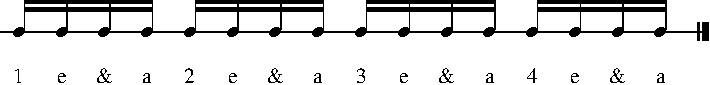
\includegraphics[width=\linewidth]{ly/u1_counts.cropped.pdf}
\end{minipage}\hfill
\begin{minipage}[t]{0.54\textwidth}\vspace{0pt}\small
Every beat has four slots: \textbf{1 e \& a}. Count all four out loud even when nothing plays on them. A rest is a slot you say but don't play.
\end{minipage}\par\vspace{4pt}
\score{u1_cells}
{\small \textbf{Cells.} Each cell is one beat long (c9 is two). These are the rhythm building blocks of the whole score. Clap each one 4 times at 56, counting. Then find them in bars 5--12 and write the cell number in pencil above each beat. Most beats are one of these nine.}

\sd{1b}{The left hand as written}
\score{u1_lh}
{\small Fingers: 5-3-1 on every chord. The pedal: press as the chord sounds, then lift and press again exactly when the next chord sounds. You should hear no gap and no blur. G (G-B-D) and Bm (B-D-F\sh) are the ledger-line chords; name their notes out loud until you stop counting lines.}

\sd{1c}{The melody, one phrase at a time}
\small
The verse is four 2-bar phrases: \textbf{5--6, 7--8, 9--10, 11--12}. Learn one phrase every few days, in four steps. Don't skip to step 4.\par\vspace{2pt}
\renewcommand{\arraystretch}{1.25}
\begin{tabularx}{\textwidth}{@{}l X@{}}
\textbf{Step 1} & \textbf{Clap and count} the phrase's rhythm, using the cell numbers you pencilled in.\\
\textbf{Step 2} & \textbf{Say the note names} in rhythm, without playing.\\
\textbf{Step 3} & \textbf{Find the hand position.} Put the finger that fits on the phrase's first note and pencil its number in. Check the highest and lowest note fit without jumping.\\
\textbf{Step 4} & \textbf{Play} right hand alone at 40, then 48, then 56.\\
\end{tabularx}\normalsize

\begin{fivemin}
\tm{0:00--1:00} & \textbf{Cells.} Two cells from 1a, 4 times each, counting aloud.\\
\tm{1:00--3:00} & \textbf{Split drill of the day}: 1b on day 1, 1c on day 2, 1d on day 3 (next page), then repeat.\\
\tm{3:00--5:00} & \textbf{The bars.} Today's phrase from 1c, hands separately, then hands together if it's ready.\\
\end{fivemin}

\newpage
%===================================================== UNIT 1b
\unit{1}{Verse, bars 5--12: rejoin}{Where the hands meet, then the two hands together.}{1a--1c}{together points}{L5}

\sd{1d}{Together points}
\score[0.87\textwidth]{u1_together}
{\small Practice material: the verse chords under a right hand on one note, with the kinds of rhythm the verse uses. The chords always fall on beats 1 and 3. The right hand often comes in on the ``\&'' or the ``e''. Count out loud; the chord and your ``one'' land together.}\par\vspace{3pt}
{\small\textbf{In your score:} draw a light vertical line through both staves at every left-hand chord (beats 1 and 3). At each line, ask: what is the right hand doing here? Often a rest, sometimes a note that starts with the chord. Those lines are the only places the hands have to agree.}

\begin{rejoin}
\item \textbf{Skeleton.} Left hand plus only the right-hand notes that sit on a line. Slow, at 40.
\item \textbf{One phrase}, hands together, 40. Then the same phrase at 48.
\item \textbf{Chain two phrases}: 5--8, then 9--12. The bar lines between phrases are where people stop, so play over them without a break.
\item \textbf{Bars 5--12}, hands together. Then climb to 56.
\end{rejoin}

\begin{ladder}
\lv{L1}{All nine cells clapped with counts}{56}
\lv{L2}{Left hand, bars 5--12, with pedal, no stops}{56}
\lv{L3}{Right hand, phrases 5--6 and 7--8}{40}
\lv{L4}{Right hand, bars 5--12}{48}
\lv{L5}{\textbf{Gate.} Hands together, bars 5--12}{44}
\lv{L6}{Same at the written tempo}{56}
\lv{L7}{Bars 5--12 along with the recording's verse}{record}
\end{ladder}

\bottomb{Play bars 5--12 without pedal and keep the chords connected with your fingers. Then with pedal again: hear the difference. Say the counts out loud while playing hands together.}
{Rhythm wrong: back to 1a and clap the phrase. Chord slow to find: 1b alone, or Drill 2 of your earlier packet. Hands collide: step 1 of the rejoin, at 40.}

\newpage
%===================================================== UNIT 2
\unit{2}{Chorus, bars 13--20 (easy)}{New chord shapes that barely move, a higher melody, and a left hand that pulses in quarters.}{Unit 1 L5}{moving shapes, ledger lines above, triplet, LH quarters}{L5}

\begin{inbars}
\textbf{Left hand:} no longer root position. C, G, Em and D are voiced so the hand stays in one place (the shapes below). Bars 13, 17 and 19 are half notes; in 14--16, 18 and 20 some chords repeat as quarter notes, so the left hand pulses on the beat. Bars 17 and 20 use \textbf{Cmaj7} (C-E-G-B), C major with B on top.\par
\textbf{Right hand:} higher than the verse, up onto the ledger lines above the staff. The same short rhythm keeps coming back: find it in bar 13 and look for it everywhere else. Bar 16 has a \textbf{triplet}.\par
\textbf{Repeats:} compare 13--16 with 17--20 before you learn anything.
\end{inbars}

\sd{2a}{The chorus hand shapes}
\begin{minipage}[t]{0.62\textwidth}\vspace{0pt}
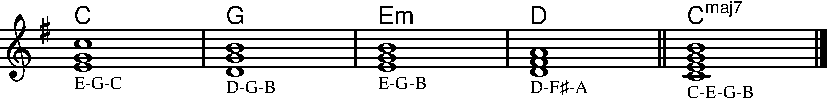
\includegraphics[width=\linewidth]{ly/u2_shapes.cropped.pdf}
\end{minipage}\hfill
\begin{minipage}[t]{0.35\textwidth}\vspace{0pt}\small
C $\rightarrow$ G: E down to D, C down to B, G stays.\\
Em $\rightarrow$ D: all three notes step down.\\
Cmaj7: root-position C plus finger 5 on B.\\
Fingers: 1-2-5 for E-G-C, 1-3-5 for the rest; Cmaj7 1-2-3-5.
\end{minipage}

\sd{2b}{Ledger lines above the staff}
\begin{minipage}[t]{0.5\textwidth}\vspace{0pt}
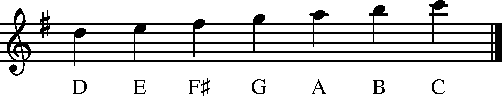
\includegraphics[width=\linewidth]{ly/u2_ledger.cropped.pdf}
\end{minipage}\hfill
\begin{minipage}[t]{0.46\textwidth}\vspace{0pt}\small
Count up from the top line (F\sh): G sits just above it, A is on the first ledger line, B sits above that, C is on the second ledger line. Quiz: point at any note in bars 13--20 and name it within 2 seconds.
\end{minipage}

\sd{2c}{New cells}
\begin{minipage}[t]{0.6\textwidth}\vspace{0pt}
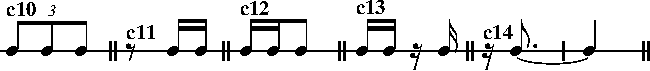
\includegraphics[width=\linewidth]{ly/u2_cells.cropped.pdf}
\end{minipage}\hfill
\begin{minipage}[t]{0.37\textwidth}\vspace{0pt}\small
\textbf{c10} is the triplet: three even notes in one beat. Say ``tri-po-let''. Pencil the cell numbers above bars 13--20, as in Unit 1.
\end{minipage}

\sd{2d}{Left-hand quarters under a busy right hand}
\score[0.87\textwidth]{u2_together}
{\small Practice material on one note. The left hand plays on every beat now, so it lines up with the right hand four times per bar, not two.}

\begin{rejoin}
\item Left hand, bars 13--20, with pedal. Then right hand in 2-bar phrases (13--14, 15--16, 17--18, 19--20), using the 1c steps.
\item Hands together per phrase at 40, then chain them. Then \textbf{verse into chorus}: bars 11--14, over the join.
\end{rejoin}

\begin{ladder}
\lv{L1}{Left hand, bars 13--20, with pedal}{56}
\lv{L2}{Ledger-note quiz: any note in 13--20 in 2 seconds}{---}
\lv{L3}{Right hand, bars 13--16}{44}
\lv{L4}{Right hand, bars 13--20}{48}
\lv{L5}{\textbf{Gate.} Hands together, bars 13--20}{44}
\lv{L6}{Verse and chorus, bars 5--20}{50}
\lv{L7}{Bars 5--20 at the written tempo}{56}
\end{ladder}

\bottomb{Make the melody louder than the left-hand chords: the chorus is where the tune has to sing. Play bars 13--20 with the left hand an octave lower.}
{Hands collide on the quarters: 2d at 40, then Drill 6 (S2) of your earlier packet. Lost on ledger lines: 2b daily for a week.}

\newpage
%===================================================== UNIT 3
\unit{3}{Intro and ending, bars 1--4 and 20--22 (easy)}{Two notes at once in the right hand, an octave higher than written. After this unit you have the whole easy version.}{Unit 1 L5}{sixths, 8va, tied notes, a 2/4 bar}{L5}

\begin{inbars}
\textbf{Right hand:} two notes at a time, mostly \textbf{sixths}, under an \textbf{8va} line: play everything under the dashed line one octave higher than written, until the line ends after bar 4. Lots of ties: a note starts before the beat and holds across it, so the beat itself is silent (the same idea as the push in your earlier packet).\par
\textbf{Left hand:} the same root-position chords as the verse. You know it already.\par
\textbf{Repeats:} bars 3--4 repeat bars 1--2. You're learning two bars, not four.\par
\textbf{Ending:} the Cmaj7 in bar 20 is tied through bar 21, which has only 2 beats (2/4), then bar 22 holds the final chord.
\end{inbars}

\sd{3a}{Sixths in G major}
\score[0.85\textwidth]{u3_sixths}
{\small Keep the hand shape fixed and move the whole hand one step at a time. Listen for the warm sound. It's a thirds drill too: a sixth is a third turned upside down.}

\begin{minipage}[t]{0.5\textwidth}
\sd{3b}{Reading 8va}
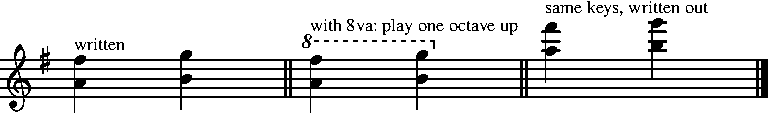
\includegraphics[width=0.95\linewidth]{ly/u3_8va.cropped.pdf}\par
{\small Read the note names as written, then move your hand up one octave. Pencil ``8va up!'' at the start of bar 1.}
\end{minipage}\hfill
\begin{minipage}[t]{0.46\textwidth}
\sd{3c}{The 2/4 bar}
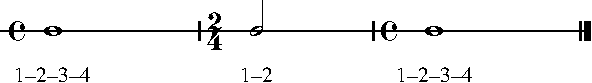
\includegraphics[width=0.75\linewidth]{ly/u3_meter.cropped.pdf}\par
{\small Bar 21 has two beats. Count ``1--2'' and move on; the final chord comes early.}
\end{minipage}

\sd{3d}{Tied notes}
\score[0.7\textwidth]{u3_ties}
{\small Clap only where a new note starts; a tie means hold, don't replay. Count every slot aloud. When a note is tied over a beat, you'll feel the urge to play on the beat. Don't.}

\begin{rejoin}
\item Right hand, bars 1--2 in the right octave: top notes only first, then both notes.
\item Hands together 1--2, then 1--4, then \textbf{1--6}: the intro into the verse. Then the ending, bars 19--22.
\item \textbf{The whole easy version}, bars 1--22.
\end{rejoin}

\begin{ladder}
\lv{L1}{Sixths up and down, one octave, right hand}{60}
\lv{L2}{3d clapped with counts}{56}
\lv{L3}{Right hand, bars 1--2, at the right octave}{40}
\lv{L4}{Right hand, bars 1--4}{48}
\lv{L5}{\textbf{Gate.} Hands together, bars 1--6 (intro into verse)}{44}
\lv{L6}{Ending, bars 19--22, hands together}{44}
\lv{L7}{\textbf{The easy version}, bars 1--22, no stops}{56}
\end{ladder}

\bottomb{Play the intro's top notes only while your left hand plays; that's your melody check. Play bars 1--22 along with the recording.}
{Wrong octave or lost place: pencil the 8va reminder. Ties get replayed: 3d at 40. Sixths feel wide: 3a daily, hands alone.}

\newpage
%===================================================== UNIT 4
\unit{4}{Normal version: intro and verse, bars 23--34}{Same melody, new hands: 16th arpeggios in the left hand, a fuller right hand.}{Unit 3 L7}{bass clef, 16th arpeggios, octave melody, clef changes}{L5}

\begin{inbars}
\textbf{Bars 23--25} are bars 1--3 again. \textbf{Bar 26} adds a left-hand chord and a quick three-note pickup, and the left hand switches to \textbf{bass clef}.\par
\textbf{Left hand, 27--34:} 16th-note arpeggios, one per chord, two chords per bar. Each climbs from a low root through the chord and back, spanning more than an octave. Bar 34 climbs back up into treble clef as a run into the chorus.\par
\textbf{Right hand, 27--34:} the verse melody from bars 5--12, with some notes doubled in octaves and chord notes added.\par
\textbf{Clefs:} the left hand changes clef in bars 26, 34 and 36. Circle each change.
\end{inbars}

\sd{4a}{Bass clef landmarks}
\score[0.75\textwidth]{u4_bassnotes}
{\small Lines from the bottom: G B D F\sh\ A. Spaces: A C E G. Learn the three Es; the verse arpeggios start from them.}

\sd{4b}{The arpeggio shape}
\score{u4_arp}
{\small Practice material with the same hand motion as your score: root, fifth, octave, tenth, and back. Fingers 5-2-1 for root-fifth-octave, then shift or stretch for the tenth. Pencil your score's fingering in once this feels natural. Change the pedal with every chord.}

\begin{minipage}[t]{0.47\textwidth}
\sd{4c}{Octaves}
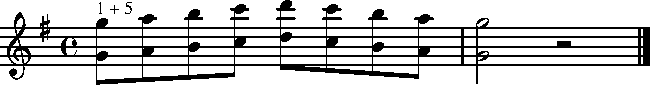
\includegraphics[width=0.95\linewidth]{ly/u4_octaves.cropped.pdf}\par
{\small Thumb and pinky, wrist loose, hand shape fixed.}
\end{minipage}\hfill
\begin{minipage}[t]{0.5\textwidth}
\sd{4d}{Build the right hand in layers}
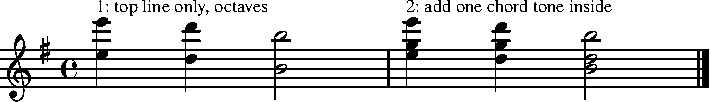
\includegraphics[width=0.95\linewidth]{ly/u4_skeleton.cropped.pdf}\par
{\small In bars 27--34: top notes only first (the melody you know from Unit 1), then the octaves, then the chord notes.}
\end{minipage}

\begin{rejoin}
\item Left hand alone, bars 27--30, at 40. Name the root of each arpeggio before you play it.
\item Right hand in layers (4d), bars 27--30. Then hands together, 2 bars at a time.
\item Bars 31--34 the same way, then \textbf{23--34}, including the clef change in bar 26.
\end{rejoin}

\begin{ladder}
\lv{L1}{Bass-clef quiz: any left-hand note in 27--34 in 2 seconds}{---}
\lv{L2}{4b round the verse chords, even 16ths}{44}
\lv{L3}{Left hand, bars 27--34}{44}
\lv{L4}{Right hand, bars 27--34, all layers}{48}
\lv{L5}{\textbf{Gate.} Hands together, bars 27--30}{40}
\lv{L6}{Bars 23--34 hands together}{48}
\lv{L7}{Same at the written tempo}{56}
\end{ladder}

\bottomb{Accent the lowest note of each arpeggio slightly: it's the bass line. Record the left hand alone and listen: are the 16ths even?}
{Arpeggio uneven: 4b at 40, or Drill 8 of your earlier packet. Lost in bass clef: 4a daily. Hands together too much: keep the right hand to top notes only for a week.}

\newpage
%===================================================== UNIT 5
\unit{5}{Normal version: chorus and ending, bars 35--44}{Two parts in one hand, a wide left hand, rolled chords and a final run.}{Unit 4 L5}{two voices, octaves and tenths, rolls, free time}{L5}

\begin{inbars}
\textbf{Bars 35--36} are close to the easy chorus (13--14). \textbf{From bar 37} the right hand carries two parts: the melody (stems up) and held chord notes (stems down). ``R.H'' marks the notes it takes. The left hand plays wide intervals in bass clef, octaves and larger, mostly as half notes. \textbf{Bar 38} has the triplet from bar 16.\par
\textbf{Ending:} bar 42 has \textbf{rolled chords} (the wavy lines) in both hands, bar 43 a \textbf{pause} (fermata), and bar 44 a fast rising run over a G chord before the last low note.
\end{inbars}

\sd{5a}{Two voices in one hand}
\score[0.82\textwidth]{u5_twovoice}
{\small Hold the lower notes with fingers 1-2 for their full length while 3-4-5 play the melody. If a held note drops early, the chord disappears. In your score, play the stems-up line alone first, then add the stems-down notes.}

\sd{5b}{Wide left hand}
\score[0.82\textwidth]{u5_wide}
{\small Octaves: fingers 5 and 1. Tenths may be too wide for your hand: roll them (bottom, then top) or leave out the top note. Both are normal.}

\begin{minipage}[t]{0.47\textwidth}
\sd{5c}{Rolled chords}
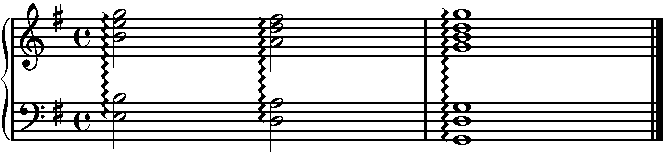
\includegraphics[width=0.8\linewidth]{ly/u5_roll.cropped.pdf}\par
{\small Bottom to top, quickly, both hands as one gesture. The top note lands on the beat.}
\end{minipage}\hfill
\begin{minipage}[t]{0.5\textwidth}
\sd{5d}{The final run}
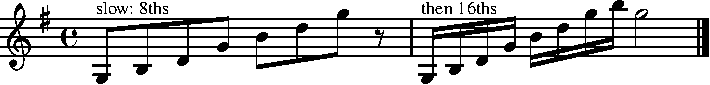
\includegraphics[width=0.95\linewidth]{ly/u5_run.cropped.pdf}\par
{\small Learn it slowly as a broken chord, then speed up. Bars 43--44 are in free time: arriving on the top note matters more than speed.}
\end{minipage}

\begin{rejoin}
\item Left hand, 37--42. Right hand, 37--38 stems-up only, then both voices. Then 39--42.
\item Hands together, 2 bars at a time, then \textbf{35--42}. Then the ending \textbf{42--44}, then \textbf{the whole normal version}.
\end{rejoin}

\begin{ladder}
\lv{L1}{5a clean, held notes full length}{56}
\lv{L2}{Left hand, bars 37--42}{48}
\lv{L3}{Right hand, bars 37--38, both voices}{40}
\lv{L4}{Right hand, bars 37--42}{44}
\lv{L5}{\textbf{Gate.} Hands together, bars 35--42}{44}
\lv{L6}{Ending, bars 42--44, with roll, pause and run}{free}
\lv{L7}{\textbf{The normal version}, bars 23--44}{56}
\end{ladder}

\bottomb{Play the whole score, easy then normal, as one 44-bar piece. Bring the melody out over the held notes in 37--41.}
{Two voices blur: 5a with the lower voice only, then add the top. LH stretch hurts: roll it or drop the top note. Rushing the ending: count the pause out loud.}

\newpage
%===================================================== TRACKER
{\fontsize{22}{24}\selectfont\bfseries Bar Tracker}\par
{\itshape Tick each box when that bar group is clean 3 times in a row. Hands separately first, then together, then at 56.}\par
\vspace{2pt}\noindent\rule{\textwidth}{0.8pt}

\sect{Bar groups}
\small
\renewcommand{\arraystretch}{1.5}
\newcommand{\bx}{\framebox(9,9){}}
\begin{tabularx}{\textwidth}{|l|l|c|c|c|c|c|X|}
\hline
\textbf{Bars} & \textbf{Section} & \textbf{Unit} & \textbf{RH} & \textbf{LH} & \textbf{Together} & \textbf{At 56} & \textbf{Notes / date}\\\hline
5--8 & Verse, first half & 1 & \bx & \bx & \bx & \bx & \\\hline
9--12 & Verse, second half & 1 & \bx & \bx & \bx & \bx & \\\hline
13--16 & Chorus, first half & 2 & \bx & \bx & \bx & \bx & \\\hline
17--20 & Chorus, second half & 2 & \bx & \bx & \bx & \bx & \\\hline
1--4 & Intro & 3 & \bx & \bx & \bx & \bx & \\\hline
20--22 & Ending & 3 & \bx & \bx & \bx & \bx & \\\hline
23--26 & Normal intro & 4 & \bx & \bx & \bx & \bx & \\\hline
27--30 & Normal verse, first half & 4 & \bx & \bx & \bx & \bx & \\\hline
31--34 & Normal verse, second half & 4 & \bx & \bx & \bx & \bx & \\\hline
35--38 & Normal chorus, first half & 5 & \bx & \bx & \bx & \bx & \\\hline
39--42 & Normal chorus, second half & 5 & \bx & \bx & \bx & \bx & \\\hline
42--44 & Normal ending & 5 & \bx & \bx & \bx & \bx & \\\hline
\end{tabularx}\normalsize

\sect{Performances}
Each is a complete run without stopping. Record it on your phone; listening back is the fastest feedback there is.\par\vspace{3pt}
\begin{ladder}
\lv{P1}{Easy verse and chorus, bars 5--20}{44}
\lv{P2}{The easy version, bars 1--22}{56}
\lv{P3}{The easy version with the recording}{record}
\lv{P4}{The normal version, bars 23--44}{44}
\lv{P5}{The normal version at the written tempo}{56}
\lv{P6}{The whole score, bars 1--44}{56}
\end{ladder}

\sect{Unit log (write the date when you tick a level)}
\small
\renewcommand{\arraystretch}{1.55}
\begin{tabularx}{\textwidth}{|l|*{7}{X|}}
\hline
\textbf{Unit} & \textbf{L1} & \textbf{L2} & \textbf{L3} & \textbf{L4} & \textbf{L5} & \textbf{L6} & \textbf{L7}\\\hline
1 Verse &&&&&&&\\\hline
2 Chorus &&&&&&&\\\hline
3 Intro \& ending &&&&&&&\\\hline
4 Normal intro \& verse &&&&&&&\\\hline
5 Normal chorus \& ending &&&&&&&\\\hline
\end{tabularx}

\end{document}
